まず, 題意のような正六角形が一つ存在するとして議論する. $L$を$x$軸とする. この正六角形は$L\subset H$をみたす平面$H$上に含まれる. $H$は実数$t$によって$z=ty$と表せるか, $y=0$ ($xz$平面)である. $S$は平面$y = 0$上では$z(x^2 + z^2) = 0$であり, これは$z=0$ ($x$軸) を表すが, この上に正六角形は作れない. 以降は平面$H: z=ty$を考える. \\
\step{1}{切断面$S\cap H$の形について}
$(x,y,ty)\in S$であるとき$y^3 + ty(x^2 + t^2y^2) = y\parenb{(1+t^3)y^2 + tx^2}$となる. $xy$平面において$y\parenb{(1+t^3)y^2 + tx^2} = 0$が表す図形$G_t$について考察する. $y = 0$は直線($x$軸)を表す. $g_t(x,y) = (1+t^3)y^2 + tx^2$が定める図形は, $a(t) = \frac{-t}{1+t^3}$ ($t\neq -1$)とおくとき
\bealn{
&g_t(x,y) = 0\\
&\iff
    \bcas
    (x,y) = (0,0)  & (\text{if} -1 < t,  0 < t)\\
    x=0 &  (\text{if} \, t=-1) \\
    y=0 &  (\text{if} \, t=0) \\
    \substack{y=0 \,\text{or}\, y=\sqrt{a(t)}x\\ \text{or}\,  y=-\sqrt{a(t)}x}  & (\text{if} -1 < t < 0)
    \ecas
}
となる. よって $t\leq -1, 0\leq t$では$G_t$が1本の直線, または2本の直線になっていることが分かる. よって$S\cap H$も2本以下の直線であるが, その上に正六角形の6頂点を取ることはできない(少なくとも3点が同一直線上にあることになってしまうため). よって\bolm{-1 < t < 0が必要である.} さらにこのとき, $G_t$はいずれも原点を通る3本の直線である. よって$S\cap H$もそのようになる.  \\
\step{2}{3直線は正六角形の最長対角線を延長したものになる}
$-1 < t < 0$のとき$S\cap H$の3直線を$L_i$($i=1,2,3$)で表すと, $L_i$は原点を共有し, 正六角形の6頂点は$L_i$のいずれかに含まれる. 正六角形の3頂点は同一直線にないので各$L_i$はちょうど2頂点を含み, どの2直線も同じ頂点を含まないことに注意し, $L_i$の位置について考察する. \par
もし$L_1$が正六角形の最長対角線を含むとすると, $L_2$は$L_1$と平行でないので辺の延長ではない. $L_2$が2番目に長い対角線を含めば, $L_3$と$L_2$が平行になるので不適. よって$L_2$も(そして$L_3$も)最長対角線を含む. このとき$L_i$は共点なのでよい. よって, $L_i$のいずれかが最長対角線を含む場合は, いずれの$L_i$も最長対角線を含む. 以降はどの$L_i$も最長対角線を含まない場合で考える. \par
$L_1$が2番目に長い対角線を含むと仮定する. その対角線の両端点の隣にある頂点を$L_i$ ($i\neq 1$)が通るとする. $L_i$は最長対角線を含まないので, 2番目に長い対角線を含む. このとき, $L_j$($j\neq 1,i$)は辺を含み, 共点ではなくなるので不適. 対称性より$L_i$はいずれも2番目に長い対角線を含まない. すると
$L_1,L_2,L_3$がいずれも辺を含む場合が残るが, この場合も共点でないので不適. よって, $L_i$は3本の最長対角線の延長であることが従う.
\begin{center}
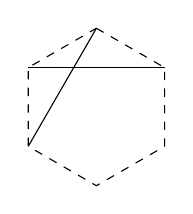
\begin{tikzpicture}
   \draw[dashed] (0,1)--({sin{60}}, {cos{60}})--({sin{120}}, {cos{120}})--({sin{180}}, {cos{180}})--({sin{240}}, {cos{240}})--({sin{300}}, {cos{300}})--cycle;
   \draw ({sin{60}}, {cos{60}})--({sin{300}}, {cos{300}});
   \draw (0,1)--({sin{240}}, {cos{240}});
\end{tikzpicture}
\end{center}
% は$S\cap H$の射影を表すので, これを$y$軸方向に$\sqrt{1+t^2}$倍拡大することで元の$S\cap H$の図が得られる. つまり, $y$を$(\sqrt{1+t^2})y$に置きなおした
% \[
% (\sqrt{1+t^2}) y \parenb{(1+t^3)(1+t^2)y^2 + tx^2} = 0
% \]
% という方程式が$xy$平面上で描く図形を$C$としたときに, $C$上の6点を結んで正六角形が作れるかを調べるとよい. そこで, $C$の形について調べる.\par
% $f_t(x,y) = (1+t^3)(1+t^2)y^2 + tx^2$とおくと, $C$は$y=0$ ($x$軸)と$f_t(x,y) = 0$で表される図形に分解する.
% $t< -1$または$0 < t$の場合は $(1+t^3)(1+t^2)$と$t$が0でなく, 同じ符号になる. よって$f_t(x,y) = 0\iff (x,y) = (0,0)$となるので, $C$は$x$軸のみになる. この場合, 正六角形を作ることは出来ない. \par
% $t=0$のとき$f_0(x,y) = y^2$なので$C$は$x$軸のみであり, 同様に不適. $t=-1$のとき$f_{-1}(x,y) = -x^2$なので$C$は$x$軸と$y$軸の和集合になるが, この場合も不適(もし作れたとすると, 9度に交わる対角線が引けることになって矛盾する). \par
% $-1 < t < 0$のとき, $m(t) = \dfrac{-t}{(1+t^3)(1+t^2)}$とおくと$m(t) > 0$であり,
% \[f_t(x,y) = (1+t^3)(1+t^2)\parena{y - \sqrt{m(t)} x}\parena{y + \sqrt{m(t)}x}\]
% となる. よって$C$は$(0,0)$を通る3つの直線$y=0$, $y=\pm \sqrt{m(t)}x$の和集合になる. \par
% (1)より, これら3直線は最長の対角線を延長したものである.
\step{3}{正六角形がただ一つ存在すること} $y=0$, $y=\pm \sqrt{a(t)} x$は$S\cap H$を$xy$平面($z=0$) に射影した直線の定義式であることに注意すると, $y$を$\sqrt{1+t^2}$倍に拡大した定義式
\[
y=0,\quad y = \pm \sqrt{1+t^2}\sqrt{a(t)}x
\]
は$S\cap H$と等長な図形となっている.
Step2.より, これらのどの2直線のなす角も60度でなければならないので, $\sqrt{(1+t^2)a(t)} = \tan{60^{\circ}} = \sqrt{3}$, すなわち
\[
4t^3 + t + 3 = 0,\quad -1 < t < 0
\]
を満たす$t$がただ一つ存在することを示せばよい. 第一式左辺を$f(t)$とおくと$f'(t) = 12t^2 + 1 > 0$なので$f(t)$は狭義単調増加で, $f(-1) = -2 < 0 < 3 = f(0)$なので, 中間値の定理により上を満たす$t$はただ一つ存在する. これを$t_0$とおく. よって,
\tbox{
題のような正六角形は, 必ず平面$H: z=t_0 y$上に含まれ, どの2本も60度で交叉する3直線$L_1,L_2,L_3$を最長対角線の延長として持つ必要がある.
}{}
3直線$S\cap H$の共点は原点${\rm O}$なので, 正六角形の中心は${\rm O}$でなければならない. よって, 上のような正六角形は, $L_i$ ($i=1,2,3$)上に${\rm OA}_{i1} = {\rm OA}_{i2} = 1$となる(異なる)2点${\rm A}_{i1}, {\rm A}_{i2}$を取ることで得られる6点を頂点とした正六角形でなければならない. この構成は一意的なので題意は示された. \qed
